% coding:utf-8

%----------------------------------------
%FOSAMATH, a LaTeX-Code for a mathematical summary for basic analysis
%Copyright (C) 2013, Daniel Winz, Ervin Mazlagic, Adrian Imboden, Philipp Langer

%This program is free software; you can redistribute it and/or
%modify it under the terms of the GNU General Public License
%as published by the Free Software Foundation; either version 2
%of the License, or (at your option) any later version.

%This program is distributed in the hope that it will be useful,
%but WITHOUT ANY WARRANTY; without even the implied warranty of
%MERCHANTABILITY or FITNESS FOR A PARTICULAR PURPOSE.  See the
%GNU General Public License for more details.
%----------------------------------------

% coding:utf-8
\section{Kurvendiskussion}

\subsection{Tangentengleichnung}
\label{subsec:tangentengleichung}
\[ \boxed{T(x) = f'(x_0)(x - x_0) + f(x_0)} \]

\subsection{Normale zur Tangente}
\[ \boxed{ T(x) = \frac{-1}{f'(x_0)} \cdot (x-x_0) + f(x_0) } \]

\subsection{Steigen und Fallen}
\label{subsec:monotonie}
\[ \boxed{ \begin{array}{lll}
f'(x) \geq 0 \text{ auf } I & \Rightarrow  
& f \text{ ist monoton wachsend in $I$} \\
f'(x) \leq 0 \text{ auf } I & \Rightarrow  
& f \text{ ist monoton fallend in $I$} \\
f'(x) > 0 \text{ auf } I & \Rightarrow  
& f \text{ ist streng monoton wachsend in $I$} \\
f'(x) < 0 \text{ auf } I & \Rightarrow  
& f \text{ ist streng monoton fallend in $I$}
\end{array} } \]

\noindent
$I$ entspricht einem Intervall! Dies bedeutet, ist $f'(x)$ über den gesamten 
Bereich immer $\geq 0$ so ist $f$ monoton wachsend. Ist $f'(x)$ über den 
gesamten Bereich $\leq 0$ so ist sie monoton fallend.

\subsection{Krümmungsverhalten}

\[ \boxed{ \begin{array}{lll}
f''(x) > 0 \text{ auf } I & \Rightarrow  
& \text{ Kurve ist konvex bzw. linksgekrümmt} \\
f''(x) < 0 \text{ auf } I & \Rightarrow  
& \text{ Kurve ist konkav bzw. rechtsgekrümmt}
\end{array} } \]

\subsection{Extremum}
Ein Extremum ist ein Punkt, zu welchem die Ableitung $0$ ergibt.
Solch ein Extremum kann ein Maximum oder Minimum sein.
Zusätzlich ist zu definieren, ob es sich um ein lokales oder globales Extremum 
handelt.

\[ \boxed{ \begin{array}{lll}
f'(x_0) = 0 \land f''(x_0) < 0 & \Rightarrow & \text{lokales Maximum in $x_0$}\\
f'(x_0) = 0 \land f''(x_0) > 0 & \Rightarrow & \text{lokales Minimum in $x_0$} 
\end{array} } \]

\subsection{Wendepunkt}
Als Wendepukt bezeichnet man jene Stelle, an welcher die Krümmung der Funktion 
wechselt (konkav zu konvex und umgekehrt).
Im Wendepunkt ist die Steigung jeweils von beiden Seiten aus betrachtet 
(d.h aus $x_0 > 0$ und $x_0<0$) extremal.

\subsubsection{Notwendiges Kriterium}
\[ \boxed{ \begin{matrix}
\text{Wendepunkt in $x_0$} & \Rightarrow & f''(x_0) = 0
\end{matrix} } \]

\subsubsection{Hinreichendes Kriterium}
\[ \boxed{ \begin{matrix}
f''(x_0) = 0 \land f'''(x_0) \neq 0 & \Rightarrow & \text{Wendepunkt in $x_0$}
\end{matrix} } \]
Achtung: Ist die dritte Ableitung 0, so kann an dieser Stelle trotzdem ein 
Wendepunkt sein. 

\subsection{Sattelpunkt}
Ein Sattelpunkt ist ein Wendepunkt mit horizontaler Wendetangente.

\[ \boxed{ \begin{matrix}
f'(x_0) =  f''(x_0) = 0 \land f'''(x_0) \neq 0 & \Rightarrow 
& \text{Sattelpunkt in $x_0$}
\end{matrix} } \]

\begin{figure}[h!]
\centering
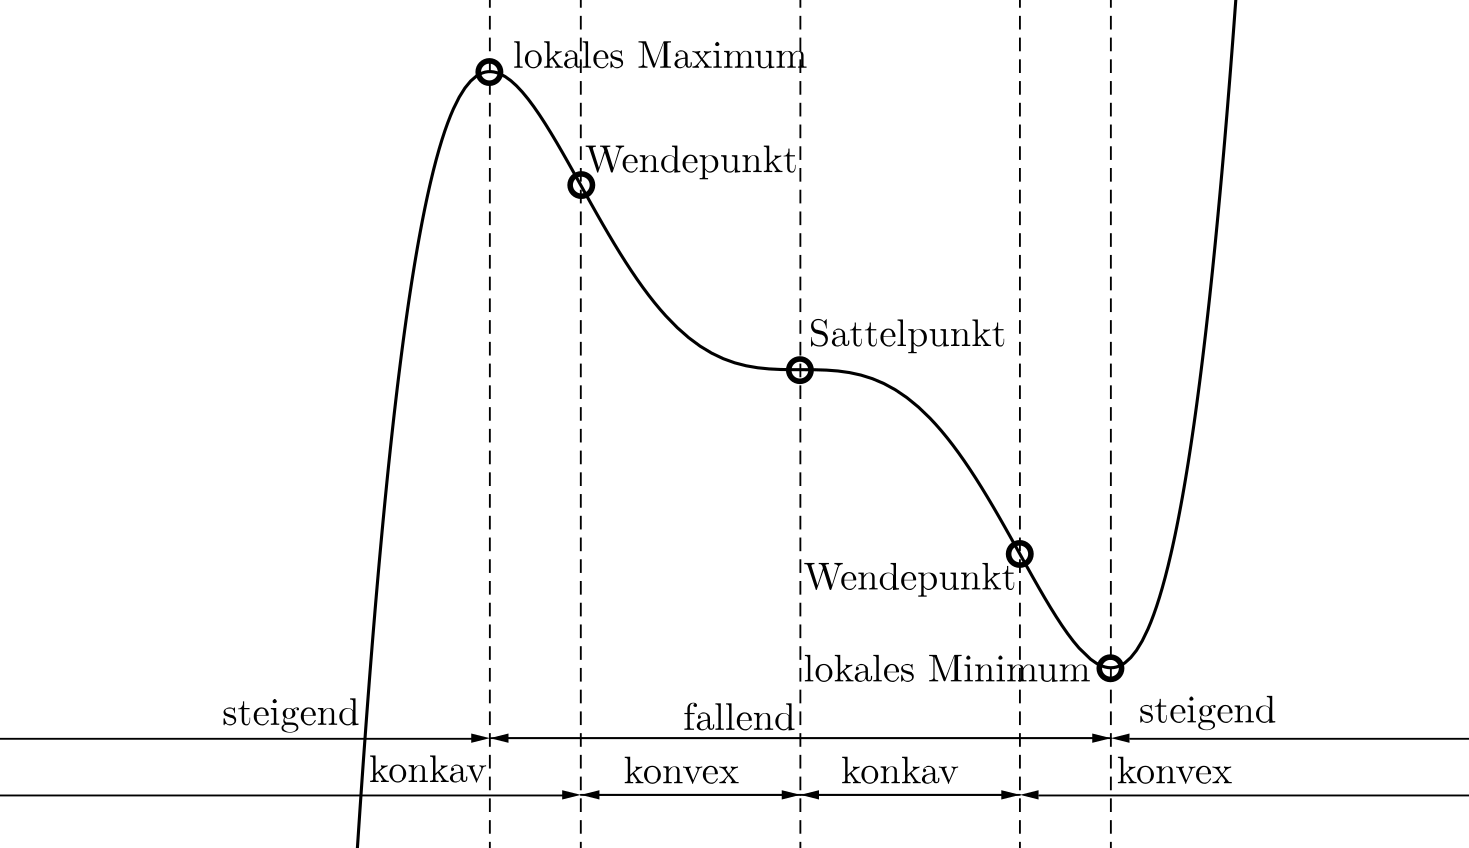
\includegraphics[width=0.88\textwidth]{kurvendiskussion.pdf}
\end{figure}
